%------------------------------------------------
% Formal Scientific Paper Template
% Sam Dougherty
% Last edited 12.2.2015
%------------------------------------------------

\documentclass[10pt,letterpaper]{article}

%------------------------------------------------
% 		Preamble
%------------------------------------------------
\title{A fitting whitty title: with colon}
\author{This guy}
\date{\today} %or put in what ever you want

%------------------------------------------------
% 		Packages
%------------------------------------------------
\usepackage{geometry}  					% For paper options
%\usepackage[parfill]{parskip}    		% Activate to begin paragraphs with an empty line rather than an indent
\usepackage{graphicx}					% For graphics
\usepackage{setspace}					% For setting spacing \doublespace, \singlespace, etc
\usepackage{fullpage}					% Makes margins equal
\usepackage[section]{placeins}			% Controls placement of floats. delete [section] and use \FloatBarrier 
\usepackage[round]{natbib}				% Citation style
\usepackage{multicol}					% For multiple columns

%------------------------------------------------
%	Setup of things
%------------------------------------------------
\geometry{letterpaper}    				% Paper size
%\geometry{landscape}                	% Activate for for rotated page geometry
\parskip=5pt
\setlength{\textfloatsep}{10pt plus 1.0pt minus 2.0pt}

%------------------------------------------------------------------------------------------------------------------------------------------------
%	This is the beginning
%------------------------------------------------------------------------------------------------------------------------------------------------
\begin{document}
\maketitle							% Title	
\tableofcontents					% TOC
%------------------------------------------------
%	Abstract
%------------------------------------------------
\begin{abstract}					% Abstract
\textit{This is abstract in a way i could never imagine. yadda yadda yadda yadda yadda yadda 
yadda yadda yadda yadda yadda yadda yadda yadda yadda yadda yadda yadda yadda yaaaaaaaaaaahh.}
\end{abstract}

%------------------------------------------------
%	Introduction
%------------------------------------------------
%SPACING
%\doublespace
% for multiple collumns
%\begin{multicols}{2}

\section{Introduction}				% Introduction
	\subsection{First Part}
	
yadda yadda yadda yadda yadda yadda yadda yadda yadda yadda yadda yadda yadda yadda yadda 
yadda yadda yadda yadda yadda yadda yadda yadda yadda yadda yadda yadda yadda yadda yadda.
	\subsection{Second Part}

yadda yadda yadda yadda yadda yadda yadda yadda yadda yadda yadda yadda yadda yadda yadda 
yadda yadda yadda yadda yadda yadda yadda yadda yadda yadda yadda yadda yadda yadda yadda.
%------------------------------------------------
%	Other Sections, results, discussion, methods etc.
%------------------------------------------------

\section{OTHER SECTION}
\begin{figure}						% Figure Example
	\centering
		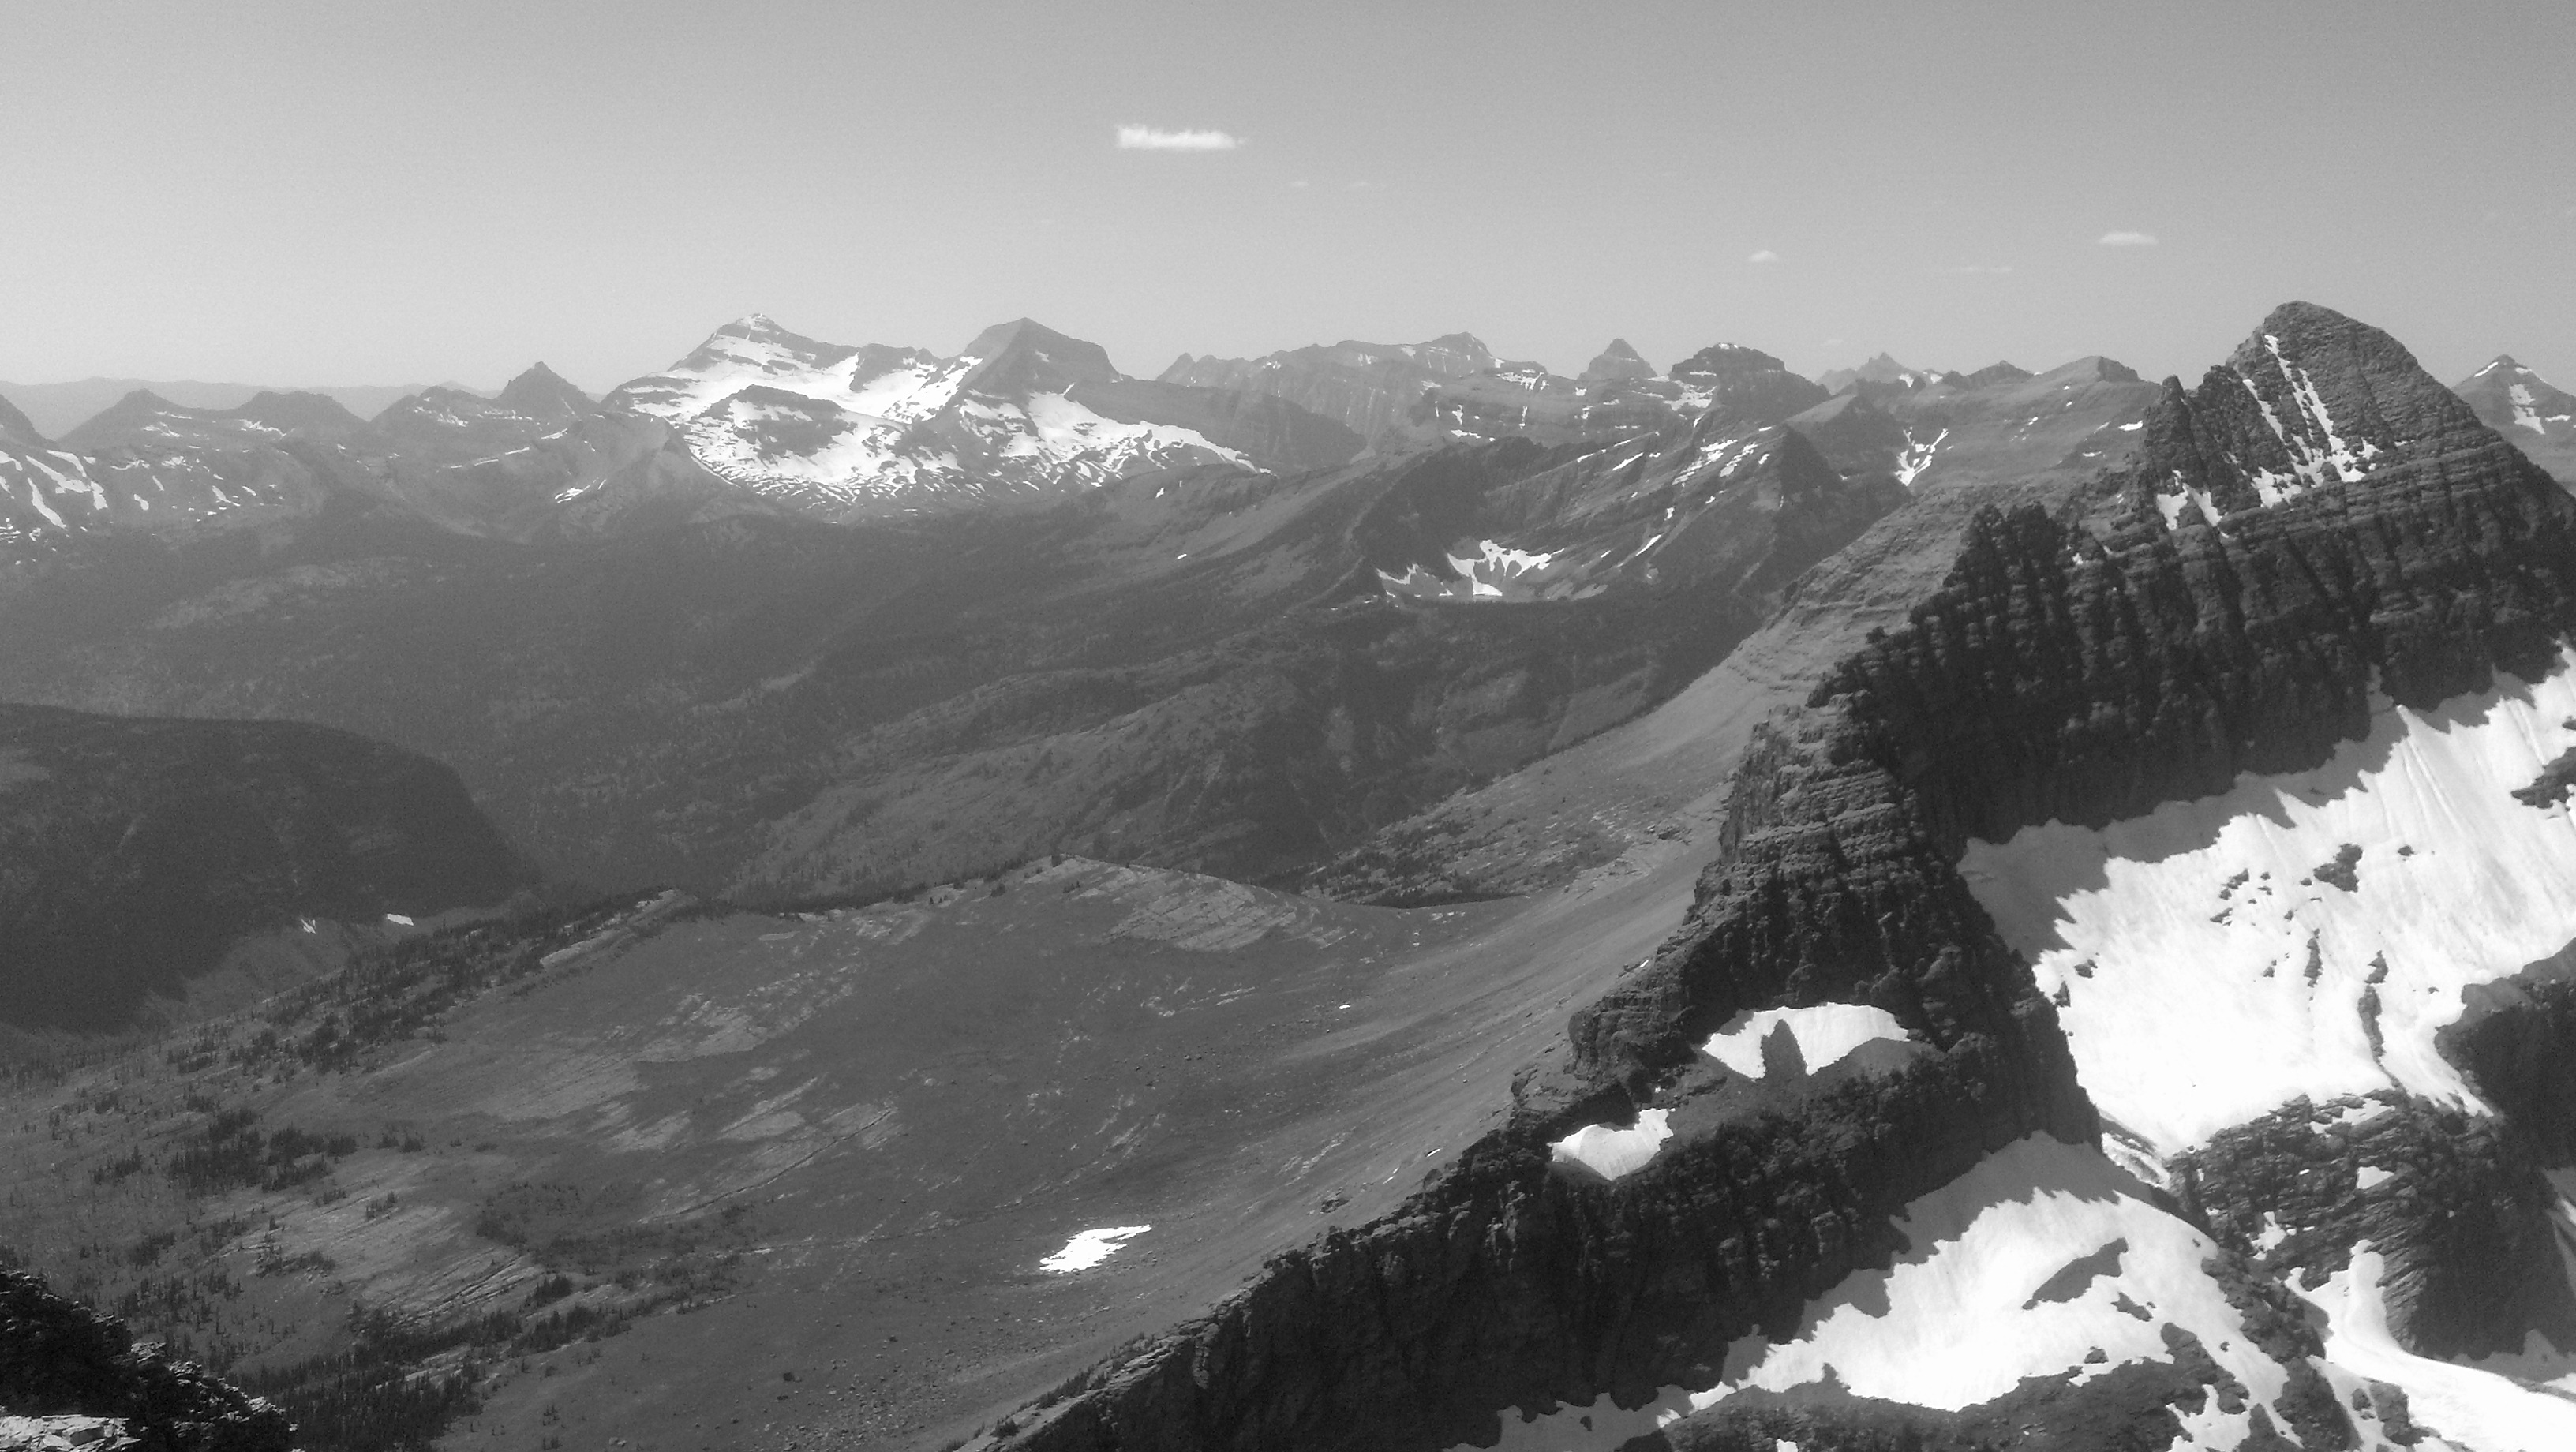
\includegraphics[width=\textwidth]{ya}
		\caption{a wonderful view of the N. Fork region in Glacier NP}   
	\vspace{.5in}
\end{figure}

%------------------------------------------------
%	Conclusion
%------------------------------------------------
\section{Conclusion}
 yadda yadda yadda yadda yadda yadda yadda yadda yadda yadda yadda yadda yadda yadda yadda 
 yadda yadda yadda yadda yadda yadda yadda yadda yadda yadda yadda yadda yadda yadda yadda 
 yadda yadda yadda yadda yadda yadda yadda yadda yadda yadda yadda yadda yadda yadda yadda.
In line citation \citet{hellawell2001gis}\\
I like this cite (parenthetical)\citep{hellawell2001gis}\\	
Other Cites \citet*{hellawell2001gis}\\
\citep*{hellawell2001gis}\\	
\citeauthor{hellawell2001gis}\\
\citetext{priv.\ comm.}	
%\end{multicols}
%------------------------------------------------
%	Bibilography
%------------------------------------------------
% REMEMBER: Compile paper, compile .BIB, Re compile paper. 
%It might take a few tries to get everytihng to work

\newpage
%\nocite{*}								% Shows everything in Bib database, not just cited things
\bibliographystyle{plainnat}
\bibliography{science}

\end{document}
